

% Section: IMPLEMENTATION
\subsection{Evaluation with Prototype}
\label{sec__incentivise_evaluation_prototype}


\subsubsection{Prototype Implementation}

We have implemented a prototype of the incentive-based regulation mechanism~\cite{Khan2014Prototyping} 
in Python using CouchDB~\cite{Anderson2010} database at the back-end,
and deployed it in Community-Lab testbed~\cite{CommunityLab}. 
We chose Python because the current host operating system installed on ONs in the testbed 
is OpenWRT~\cite{Openwrt}, which supports Python, but does not support many other languages such as Java. 
We selected CouchDB because among its advantages, 
it is lock-free, schema-less and provides a REST interface, 
and is also part of the other components of the SN's cloud management software being developed.
In the SNs, Debian operating system is installed. 

Figure~\ref{fig:cloud-coordinator-arch} shows the implemented components of the cloud coordinator from the architecture in \Cref{sec__cloud_arch}.
The components from the prototype are described below.

\paragraph{ON Management} 
ONs can register with SN to request and to contribute resources.

\paragraph{Regulation Mechanism} 
When pooling resources from multiple zones, 
the cloud coordinator applies a regulation mechanism 
that takes into account resource utilisation 
and contribution by different nodes to perform resource allocation. 

\paragraph{SN Interconnectivity} 
The design of a community cloud manager follows a decentralised approach, 
so cloud coordinator relies on gossip-based discovery mechanisms to manage overlay network of the SNs in community cloud. 
The updated list of adjacent SNs is saved in SN-List database.

\paragraph{SN Resource Sharing} 
When requests from ONs cannot be met from resources in the local zone, 
SN can request resources from other SNs in the system.

\paragraph{}
ONs use the remote procedure call (RPC) mechanism to connect to the SN. 
First of all, an ON assigns itself to a parent SN with a register message which includes metadata of that ON such as IP address, total capacity and number of VMs shared. 
In the current prototype, the IP address of SN is fixed and is manually provided when setting up ONs.
However in future, service discovery tools like Serf~\cite{Serf} can be used to get address of SN.
This registration information is stored in the ON-List database of the parent SN by creating an entry for the corresponding ON. 
After that, the ON is ready to send requests to its parent SN, 
which are processed using Algorithm~\ref{fig__incentives_algo_request_processing}
as shown in Figure~\ref{fig:sequence-dig-controller-request}.
When an ON requests its parent SN for any VMs, it specifies the duration for how long it needs to use the VMs. 
This request is evaluated by performing incentive and decision mechanisms as explained in section~\ref{sec__incentives_design}. 
If a request cannot be met locally, the corresponding parent SN checks its SN-List database to find another zone with available resources. 
The interactions between SNs are also made through RPC mechanism.
In the SN controller software, there is a separate process which regularly checks the database for any updates. 
If the duration of a consumer ON's resource request has expired, 
it frees the VMs and makes them available for the provider ON, 
and updates the metadata entries of the corresponding ONs in the ON-List database.
The current implementation keeps track of the number of VMs contributed and consumed by each ON. 
The system copes with ONs connecting and disconnecting from the SN at any time since ONs periodically send heartbeat messages to the SN. 
The design allows us to include values of metrics like CPU, memory, and bandwidth usage in the future for fine-grained decisions about resources assignment. 

%% FIGURE
\begin{figure}[tbp]
\centering
	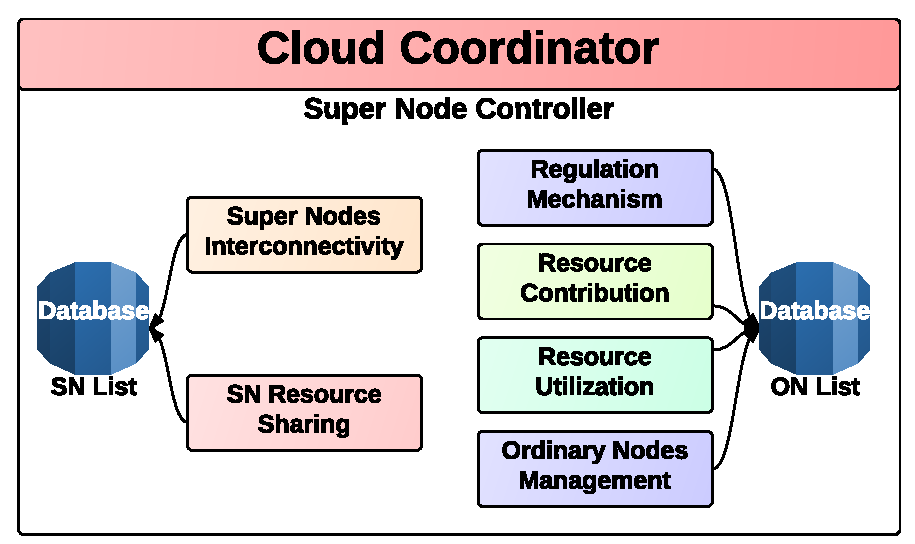
\includegraphics[width=0.75\textwidth, keepaspectratio]{vmm-cordinator-arch}
	\caption{Components of cloud coordinator}
	\label{fig:cloud-coordinator-arch}
\end{figure}